The Advanced Laser Interferometer Gravitational-Wave Observatory (aLIGO) is part of an international effort to detect gravitational waves. 
The search will resume later this year with the two aLIGO sites in Washington and Louisiana, which will ramp up to full design sensitivity over the following few years.

\section{Basic layout of aLIGO}

In its simplest form, aLIGO is a Michelson interferometer with Fabry-P\'erot cavities for arms (see figure \ref{fig:michelson}). In each Fabry-P\'erot cavity, the mirror closer to the Michelson beam splitter is called the input test mass (ITM) and the other mirror is called end test mass (ETM).

When a gravitational wave passes through the detector, it causes changes in the distance between the ETM and ITM in each cavity. Because the wave is quadrapolar, the changes in the x direction will have the opposite sign of the changes in the y direction. This causes a relative phase shift in each of the arms in opposite directions. When they recombine at the beam splitter, the phase shifts cause changes in the interference between the two beams, changing the amount of power at the the output port. We can detect these power fluctuations to reconstruct the phase shift and thus the strain, $h=\Delta L/L$ experienced by the interferometer due to the gravitational wave. We then use techniques like matched filtering to compare the strain signal from the interferometer to models of expected signals to search for events hidden in the noise background of the interferometer. 


\begin{figure}[htp]%
\center
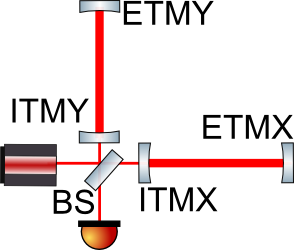
\includegraphics[width=.5\textwidth]{figures/introduction/Michelson}%
\caption[Simplified LIGO Layout]{In its simplest form, aLIGO is a Michelson interferometer with Fabry-P\'erot cavities for arms. Light from the laser is split by the beam splitter (BS), then enters the arm cavities through the input test masses (ITMX and ITMY). Power builds up in the cavity between input and end test masses (ETMX and ETMY). When a gravitational wave passes through the detector, it shifts the phases of light in the two arms in opposite directions. Because the cavity is over-coupled ($r_{ITM}<r_{ETM}$), light leaves the arm cavities and goes back to the BS. The phase-shifted light from the two cavities interferes at the BS, producing the error signal that we measure with a photodiode.}%
\label{fig:michelson}
\end{figure}

%With the goal of suppressing the noise and improving the signal, many changes have been made to the initial simple interferometer. The masses have been upgraded to 40 Kg and suspended from quadruple pendulum systems to reduce seismic noise. Mirrors have been installed for power and signal recycling to maximize the laser power in the arms. This has already led us to an increase in range by a factor of almost 3. In addition, aLIGO plans to upgrade the current input laser power from 25 watts to 125 watts, which should bring the final range of the detectors over 200 MPc. 
%
%However, an increase in laser power includes several challenges. One such effect that will scale with power is the Sidles-Sigg instability. 
%In simple terms, the Sidles-Sigg instability comes from angular or spot location displacements that cause torques on the mirrors and gets stronger as the intra-cavity power increases. 
%One mode is called the ``Hard mode'' and the other is called the ``soft'' mode. They are described in more detail in Chapter \ref{ch:application}. 
%This effect must be dealt with by using active controls on the angular degrees of freedom of the test masses.
%
%We want to develop a method to control the angular motion and damp the Sidles-Sigg instability of the ITMs and ETMs as we increase the laser power.  We know that increasing the gain of the current angular control system will result in more sensing noise being injected into the system, which may limit the sensitivity of the instrument. We think that optical springs can offer a robust control system that is not subject to sensing noise, which would be a very good solution.
%
%\section{Optical Springs}
%
%Optical spring is a term used to describe the linear region of the interaction between cavity length and radiation pressure force in a detuned Fabry-P\'erot cavity.  
%
%
%
%\begin{figure}[htbp]%
%\center
%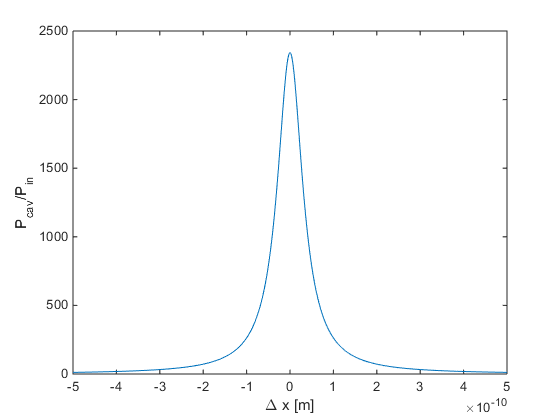
\includegraphics[width=.5\textwidth]{figures/introduction/pcav}%
%\caption[Cavity power near resonance]{Optical power in a critically coupled cavity near resonance. The height of the peak is determined by the reflectivities of the two mirrors and the }%
%\label{fig:pcav}%
%\end{figure}
%
%Radiation pressure force is given by 
%
%\begin{equation}
%F=\frac{P_{cav}}{2c}
%\label{eq:radpress}
%\end{equation}
%
%In a cavity sweeping position, we expect the power to go like (see figure \ref{fig:pcav}):
%
%\begin{equation}
%P_{cav} = P_{in} \left| \frac{t_1}{1-r_1 r_2e^\frac{-4i\pi\Delta x}{\lambda}}\right| ^2
%\label{eq:pcav}
%\end{equation}
%
%Where $t_1$ and $r_1$ are the amplitude transmisivity and reflectivity of the input mirror and $r_2$ is the reflectivity of the end mirror. $\lambda$ is the wavelength and $\Delta x$ is the displacement from the cavity resonance. 
%
%We can see that there are approximately linear regions on both sides of resonance. 
%This is the basis of a pragmatic explanation of optical spring behavior, demonstrated in figure \ref{fig:opticalsprings}.
%In this demonstration, we see the effects of ``red'' and ``blue'' detuning, where the cavity resonant length is longer and shorter, respectively, than cavity itself. 
%The color association of these detunings comes from the laser frequency shift that could accomplish this detuning: red is a negative frequency detuning and blue is a positive frequency detuning. 
%
%
%\begin{figure}[htbp]%
%\center
%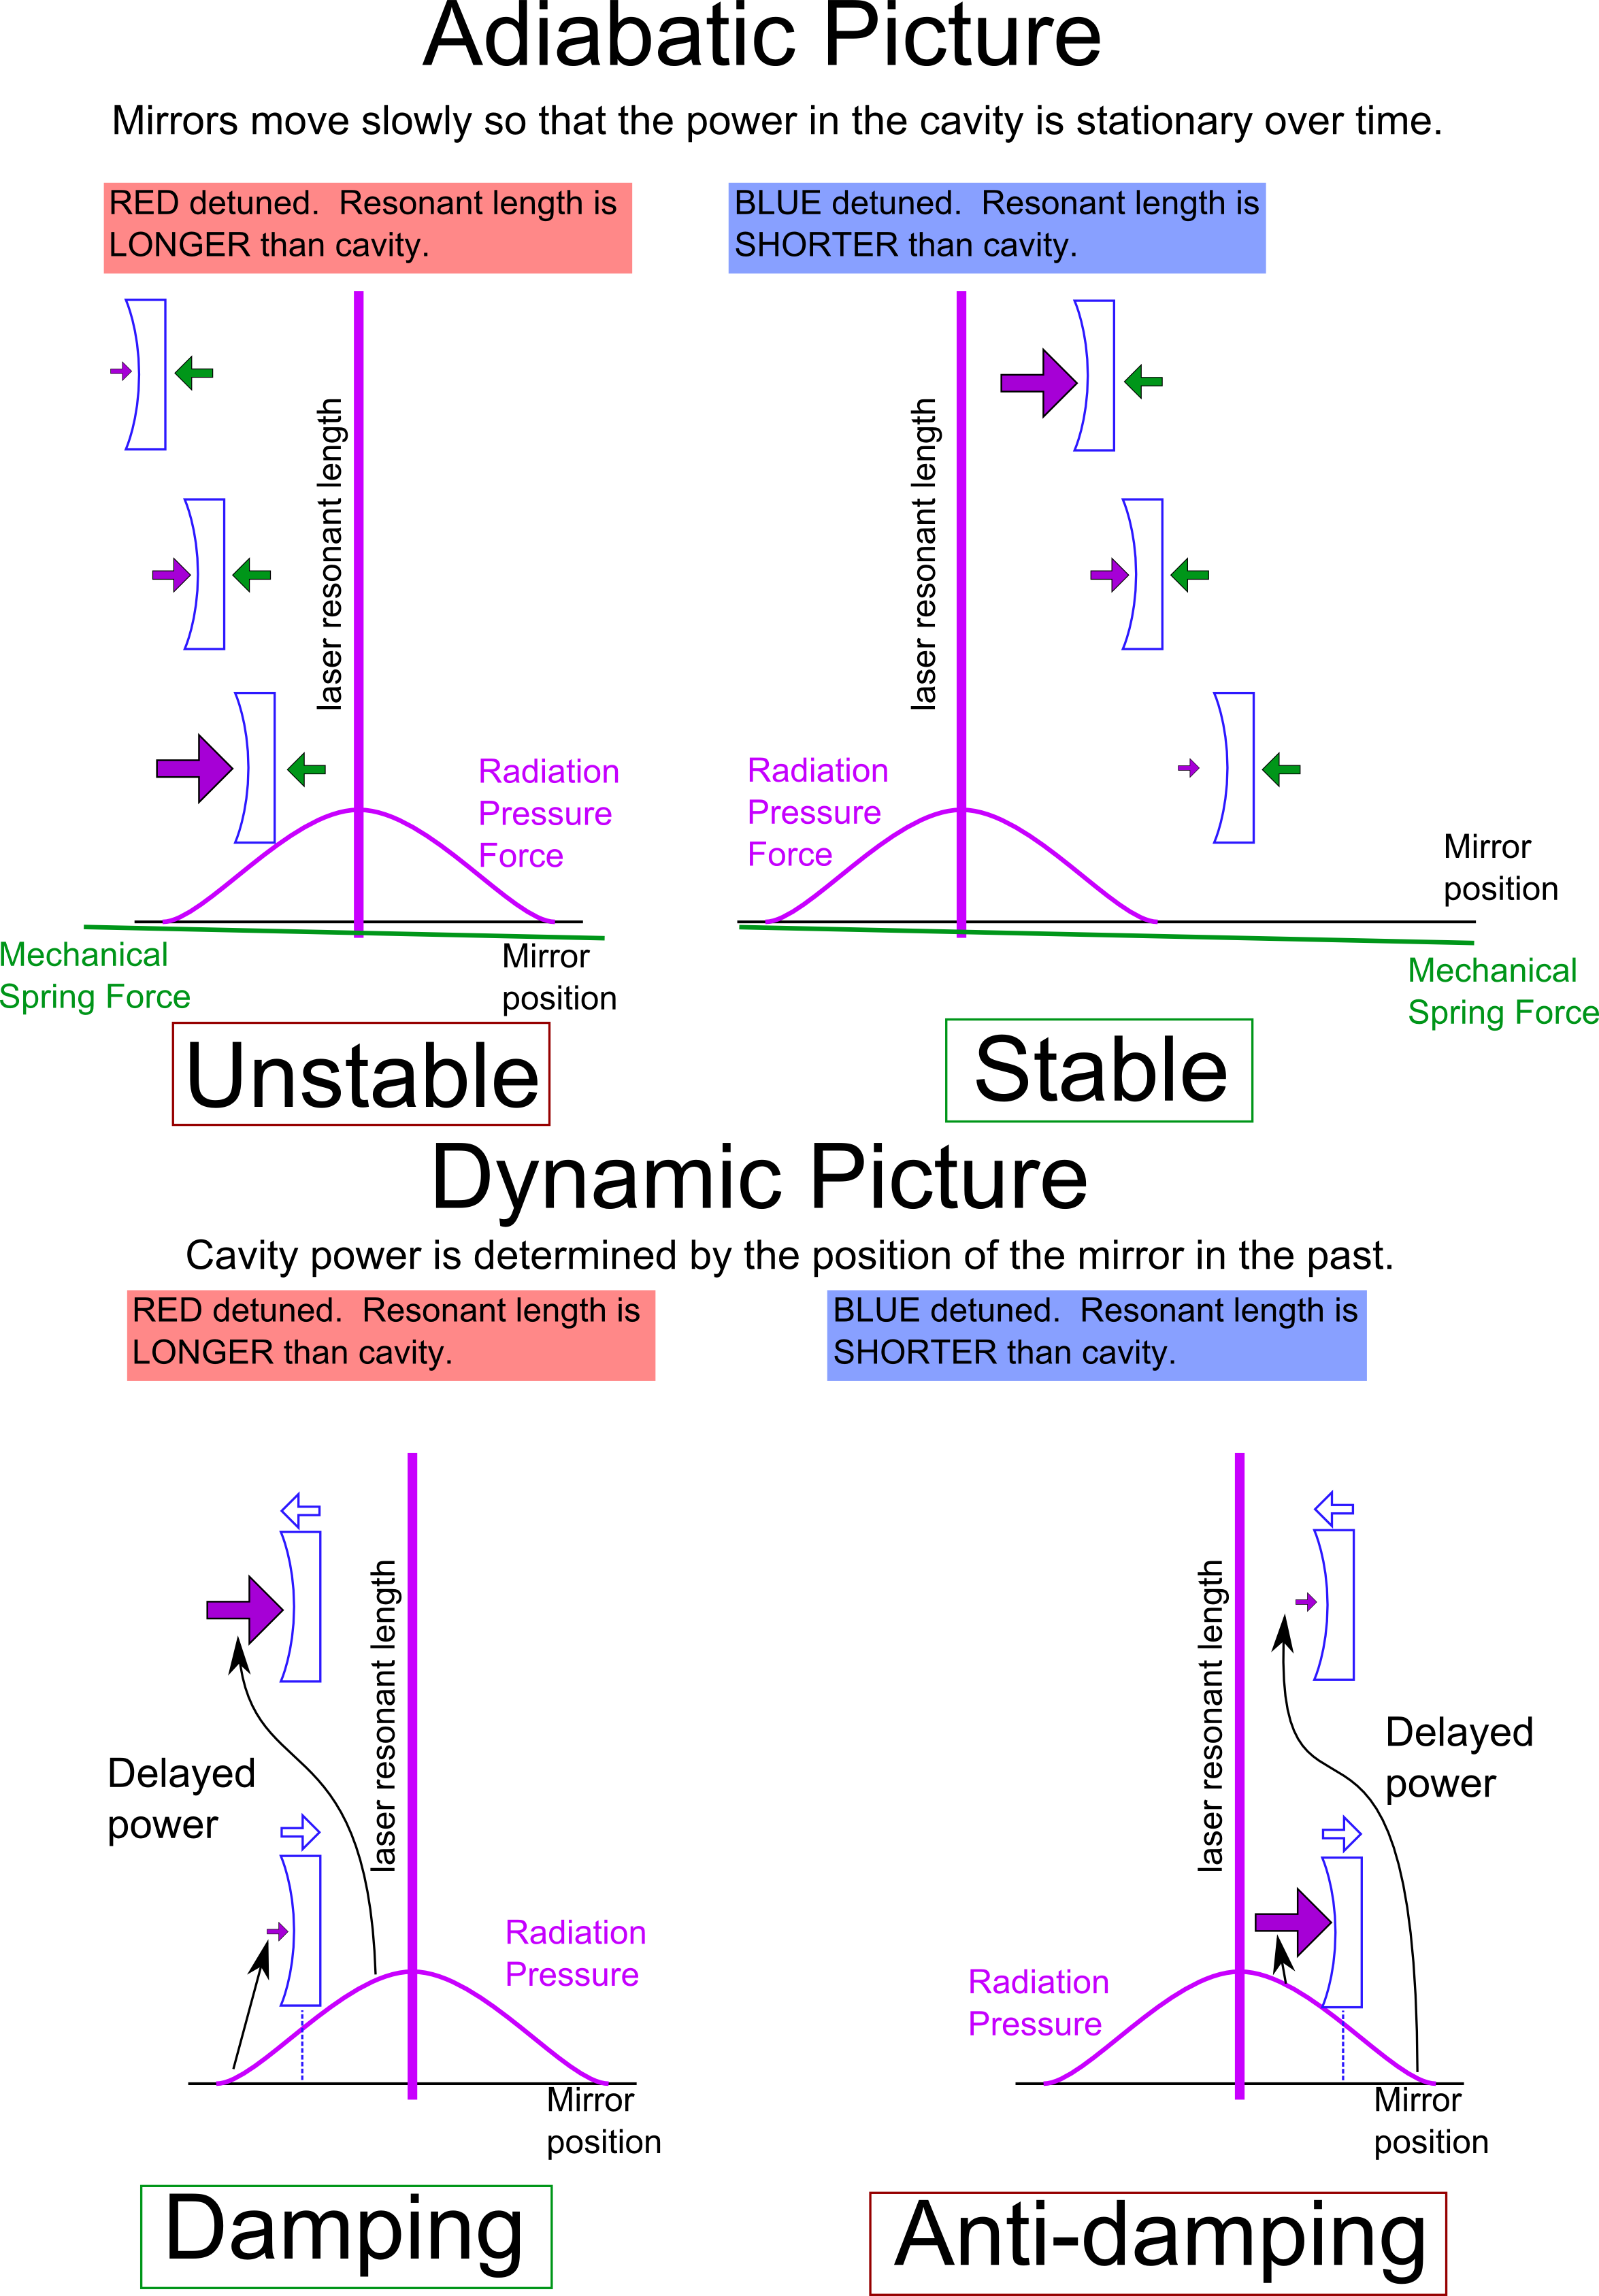
\includegraphics[width=.9\textwidth]{figures/introduction/cavity}%
%\caption[Optical spring stability]{Stability behavior of detuned cavities (optical springs). It is important to note that we rely on a constant force exerted on the mirror to choose the equilibrium point of the optical spring.}%
%\label{fig:opticalsprings}%
%\end{figure}
%
%In figure \ref{fig:opticalsprings}, we explore four different situations. For each one, I have drawn the resonant power (radiation pressure force) buildup in the cavity as a function of position. I have also shown an effectively static force due to a mechanical spring. It is important to note that we treat this as constant over position and time scales that we are dealing with.
%
%In the first case, we address a red-detuned cavity in the adiabatic, or essentially stationary, case. As the mirror moves away from its equilibrium point, it experiences more force in the direction of displacement. In the blue-detuned case, we see that the net force is pushing the mirror back to its equilibrium position. Thus the red-detuned cavity is statically unstable, while the blue-detuned cavity is statically stable.
%
%In the other case, we address a mirror that is in motion. This cavity will experience the radiation pressure force due to the position of the mirror in the recent past, determined by light travel time. In the red-detuned case, we see that the time-delayed force has an overall damping effect on the motion of the mirror. In the blue-detuned case, we get the opposite, anti-damping behavior. 
%
%In summary, we see that a blue-detuned cavity is statically stable and dynamically unstable, while a red-detuned cavity is statically unstable and dynamically stable.
%
%We can describe an optical spring as having a spring constant that follows Hook's law ($F=-kx$) in this case, we treat damping as an imaginary component to the spring constant. 
%Thus, a blue-detuned optical spring has a positive real part and a negative imaginary part, while a red-detuned optical spring has a negative real part and a positive imaginary part.
%However, since these optical springs behave like normal springs, you can add the spring constants of two of them together to arrive at a stable spring (see figure \ref{fig:opticalspringadd}).
%
%\begin{figure}[hbtp]%
%\center
%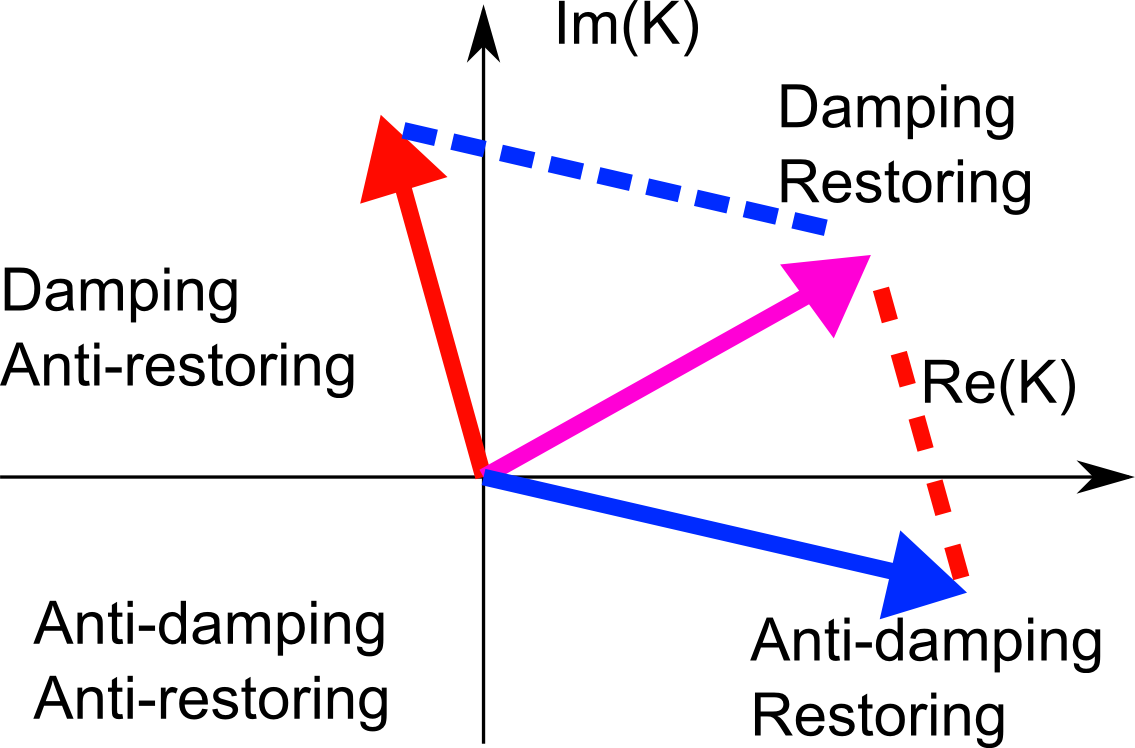
\includegraphics[width=.5\textwidth]{figures/introduction/springadd}%
%\caption[Adding Optical Springs]{We can add two unstable optical springs to make a system that is statically and dynamically stable. Note: this picture only makes sense in the low-frequency regime.}%
%\label{fig:opticalspringadd}%
%\end{figure}
%
%\section{Optical spring derivation (from Perreca 2014)}
%
%In this section we consider the effect of light stored in a detuned Fabry-Perot cavity using a classical approach.
%The intra-cavity power generates radiation pressure that exerts on the cavity mirror a force $F_{rad}=-K_{OS}\cdot x$,
%where $x$ is the mirror displacement and $K_{OS}$ is the optical spring constant.
%Here we show the full derivation of the optical spring constant $K_{OS}$.
%
%We consider a suspended Fabry-Perot cavity of length $L_0$ %shined by a laser light 
%with an incident beam of wavelength $\lambda$ and power $P_0$.
%First we calculate a general expression of the intra-cavity power and then its  radiation pressure force exerted on the end mirror.
%
%
%\begin{figure}[htbp]
	%\centering
		%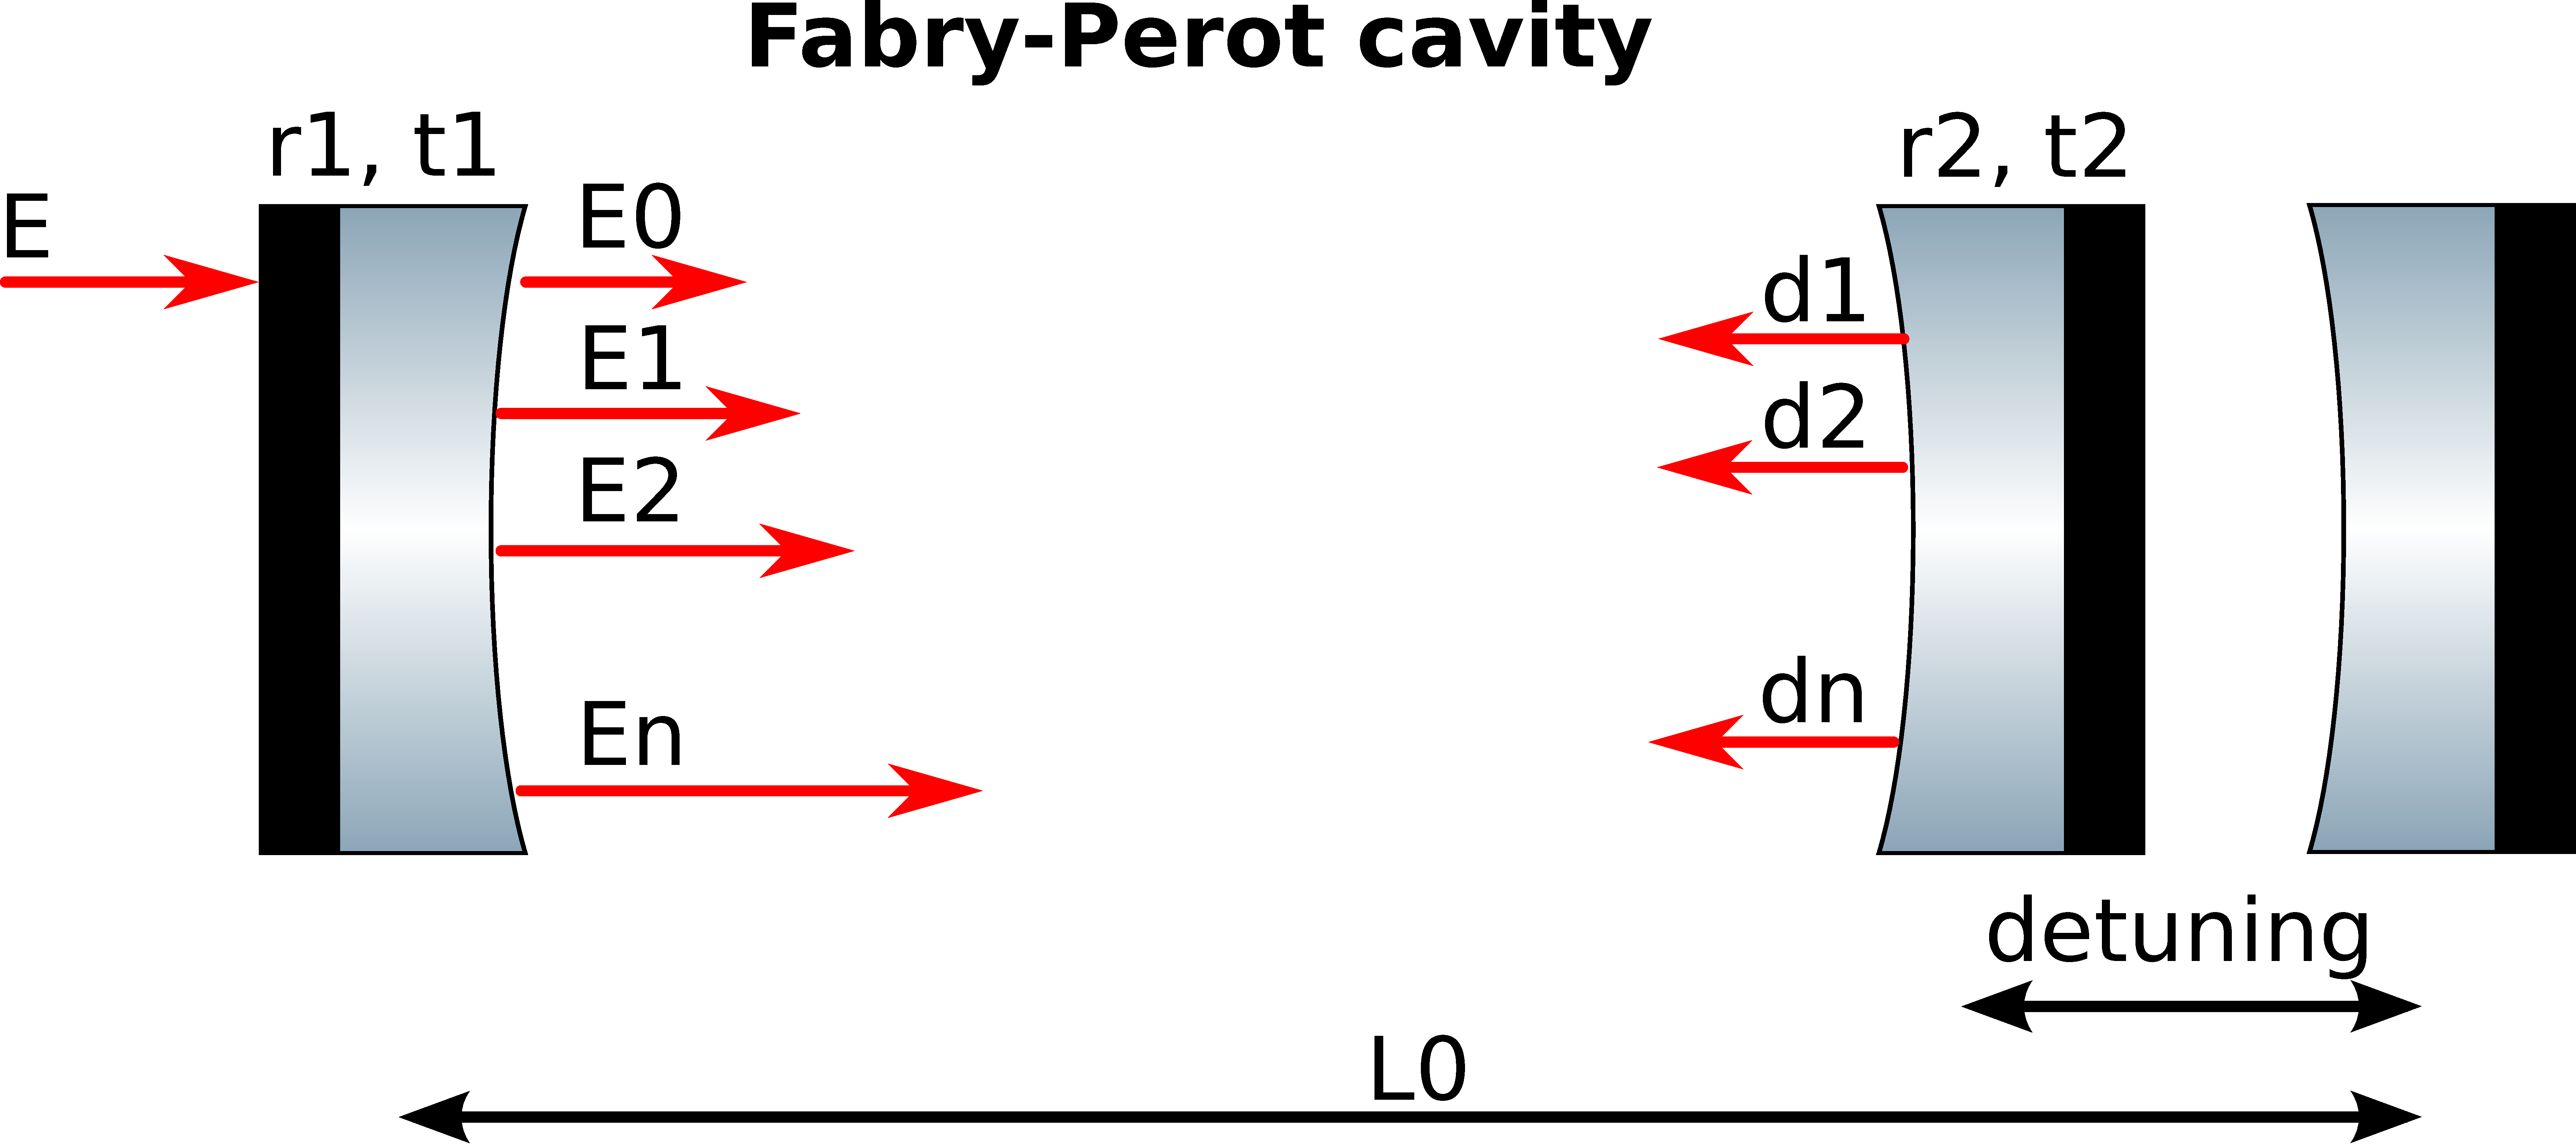
\includegraphics[width=8cm]{figures/introduction/cavitypaper}
	%\caption[Fabry-P\'erot cavity with optical spring behavior]{A Fabry-Perot cavity of length $L_0$ and coefficients $r_1,t_1$ and $r_2,t_2$ for the input and end mirrors respectively. 
	%The input mirror is stationary while the end mirror is affected by harmonic motion. The incoming field $E$ at each round-trip $i$ adds up a phase shift due to the displacement $d_i$}
	%\label{fig:cavity_k}
%\end{figure}
%
%
%The field $E=A_0e^{i\omega t}$ enters the cavity through the input mirror of coefficient $t_1=t$ and $r_1$ and the field inside the cavity at the input mirror can be seen as following
%
%\begin{align}
%E_{tot}=E_0+E_1+E_2+E_3+...+En+...
%\end{align}
%
%
%We consider in our model the following definitions, with $d_n$ being the displacement of the mirror,
%
%\begin{align}
%L_1 &= 2(L_0+d_1)\nonumber \\
%L_2 &= 2(2L_0+d_1+d_2)\nonumber \\
%L_3&=2(3L_0+d_1+d_2+d_3) \nonumber \\
%L_4 &= ...
%\end{align}
%with 
%\begin{align}
%\label{eqn:dn1}
%d_n &= d(t-[(2n-1)\tau + \alpha_n ]) \quad \mbox{and}\\
%\label{eqn:dn2}
%\alpha_n &= 2\sum\limits_{l=1}^{n-1}\frac{d_l}{c}-\frac{d_n}{c}
%\end{align}
%
%where $\tau=L_0/c$.
%With the round trip length $L=2L_0$  we obtain
%
%\begin{align}
%E_{tot}&= tE(1+r_1r_2 e^{-ikL_1}+(r_1r_2)^2 e^{-ikL_2}+(r_1r_2)^3 e^{-ikL_3}  \cdots )\nonumber \\
%&= tE(1+r_1r_2 e^{-ikL}e^{-2ikd_1}+(r_1r_2)^2 e^{-2ikL}e^{-2ik(d_1+d_2)}+(r_1r_2)^3 e^{-3ikL}e^{-2ik(d_1\!+\!d_2\!+\!d_3)}  \cdots )%\nonumber
%\end{align}
%
%
%
%If we define $X=r_1r_2 e^{-ikL}$ we have 
%
%\begin{align}
%E_{tot} = tE(1+Xe^{-2ikd_1} +X^2e^{-2ik(d_1+d_2)}
%+X^3e^{-2ik(d_1+d_2+d_3)} \cdots )%\nonumber
%\end{align}
%
%
%
%Since by definition the optical spring $K_{OS}$ is the linear term in the expansion $F=F_0+ K_{OS} d + O(d^2)$, we now expand the exponential in $d_n$. We group  $d_n$ terms:
%
%\begin{align}
%E_{tot} =& \,tE[1+X(1-2ikd_1) +X^2(1-2ik(d_1+d_2))\nonumber \\ 
%&+X^3(1-2ik(d_1+d_2+d_3)) + \cdots ]\nonumber \\ 
%=& \,tE[1+X+X^2+X^3 +\cdots\nonumber \\
%&-2ikd_1(X+X^2+X^3\cdots)\nonumber \\
%&-2ikd_2(X^2+X^3+X^4\cdots)\nonumber \\  
%&-2ikd_3(X^3+X^4+X^5\cdots)]\nonumber \\ 
%=& \,\frac{tE}{1-X}(1-2ikd_1 X-2ikd_2 X^2-2ikd_3 X^3+\cdots) %\nonumber
%\end{align}
%Since any correction from $\alpha_n$ (equation \ref{eqn:dn2}) is quadratic in $d(t)$, we can again neglect it by definition, and find for the harmonic mirror motion (i.e. in the Fourier domain)
%\begin{align}
%d_n& = x_0e^{i\Omega(t-(2n-1)\tau)}=x_0e^{i\Omega t}e^{-i\Omega(2n-1)\tau}\nonumber \\
%& = x_0e^{i\Omega t} \frac{Y^{2n}}{Y}\frac{Y}{Y}=Y^{2n-2}d_1
%\end{align}
%
%where $Y=e^{-i\Omega\tau}$. Thus we can write
%
%
%\begin{align}
%E_{tot}&=\frac{tE}{1-X}(1-2ikd_1 X-2ikd_1 Y^2X^2-2ikd_1 Y^4 X^3-2ikd_1 Y^6 X^4\cdots)\nonumber \\
%&=\frac{tE}{1-X} \left[1-2ikd_1 X(1+ Y^2X+ Y^4 X^2+Y^6 X^3\cdots)\right]\nonumber \\
%&=\frac{tE}{1-X}\left [1-\frac{2ikd_1 X}{1-Y^2X}\right ]
%\end{align}
%
%where $d_1$ is a complex number. Since we have to take its real part $Re (d_k)=\frac{d_k+\bar{d}_k}{2}$,
%we consider the field inside the cavity with $\bar{d}_k$ conjugate of $d_k$:
%
%\begin{align}
%\frac{tE}{1-X}\left [1-\frac{2ik\bar{d}_1 X}{1-\overline{Y}^2 X}\right ]
%\end{align}
%
%and we obtain as total field $E$
%
%\begin{align*}
%E_{tot}=tE\left [\frac{1}{1-X}- \frac{2ikX}{2(1-X)}   \left ( \frac{d_1}{1-Y^2 X} +\frac{\bar{d}_1}{1-\overline{Y}^2 X}\right )\right]
%\end{align*}
%
%and its complex conjugate 
%
%\begin{align*}
%\overline{E}_{tot}=t\overline{E}\left [\frac{1}{1-\overline{X}}+\frac{2ik\overline{X}}{2(1-\overline{X})}   \left ( \frac{\bar{d}_1}{1-\overline{Y}^2 \overline{X}}+\frac{d_1}{1-Y^2 \overline{X}}\right )\right]
%\end{align*}
 %
%Using the following expression
 %
%\begin{align}
%d_1=x_0e^{i\Omega(t-\tau)}=x_0e^{i\Omega t}e^{-i\Omega\tau}=xY  
%\end{align}
 %
%%Since we are interested only in the linear terms of $d_n$, 
%%we neglect $O(d^2)$ terms (\tcb{Stefan could you write a sentence here to say "WHY"?})
%we can now obtain the intra-cavity power expression by multiplying $E_{tot}$ by its conjugate
%and considering only the linear terms of $x$
%%(we neglect $O(d^2)$ terms \tcb{Stefan could you write a sentence here to say "WHY"?})
 %
%\begin{align}
%P=&E_{tot}\cdot \overline{E}_{tot}=P_0 t^2[ \frac{1}{(1-X)(1-\overline{X})}\nonumber \\  
%&-\frac{ikX xY}{(1-\overline{X})(1-X)(1-Y^2 X)} -
%\frac{ikX \bar{x}\overline{Y}}{(1-\overline{X})(1-X)(1-\overline{Y}^2 X)} \nonumber \\ 
%&+\frac{ik\overline{X} \bar{x}\overline{Y} } {(1-\overline{X})(1-X)(1-\overline{Y}^2 \overline{X})}+ 
%\frac{ik\overline{X} xY}{(1-\overline{X})(1-X)(1-Y^2 \overline{X})}]  \\ %\nonumber
%%\frac{k^2 |X|^2}{4(1-X)(1-\overline{X})} \left( 
%%\frac{|x|^2|Y|^2}{(1-Y^2 X)(1-\overline{Y}^2\overline{X})}+
%%\frac{|x|^2|Y|^2}{(1-\overline{Y}^2 X)(1-Y^2\overline{X}) }+\nonumber 
%%\frac{x^2 Y^2}{(1-Y^2 X)(1-Y^2\overline{X})}+
%%\frac{\bar{x}^2 \bar{Y}^2}{(1-\overline{Y}^2 X)(1-\overline{Y}^2\overline{X})}
%%\right) ]   
 %%\right] 
%\end{align}
%
%where we have also neglected the first constant term. We now group the terms in $x$ and $\bar{x}$:
%
%\begin{align}
%%\centering
%P=&-P_0t^2 [ \frac{ikY}{(1-\overline{X})(1-X)} \left( \frac{X}{1-Y^2 X}-\frac{\overline{X}}{1-Y^2\overline{X}} \right) x\nonumber \\
%&+\frac{ik\overline{Y}}{(1-\overline{X})(1-X)} \left( \frac{X}{1-\overline{Y}^2 X}-\frac{\overline{X}}{1-\overline{Y}^2\overline{X}} \right)\bar{x} ]\nonumber \\
%=&-P_0t^2 [ \frac{ikY}{(1-\overline{X})(1-X)} \left( \frac{X}{1-Y^2 X}-\frac{\overline{X}}{1-Y^2\overline{X}} \right) x + cc ]
%\end{align}
%Once we have calculated the power we can obtain the radiation pressure force on the end mirror by $F_{rad}=\frac{2 r_2^2}{c}P$. Furthermore
%we can also notice the similarity of the expression with the elastic force. Thus we recall that
%in frequency domain and complex notation $K$ is defined by $F=-Kx$, the real form is thus
%
%\begin{align*}
%F'=Re[F]=-\frac{1}{2}(Kx+\overline{K}\bar{x})=-\frac{1}{2}(Kx+cc)
%\end{align*}
%
%Taking into account that we are calculating the radiation pressure on the end mirror, we need to consider an extra delay factor $Y$
%for the calculation of the power which appears in the expression of $K$. The complex spring is then given by 
%
%\begin{align*}
%%\centering
%K=\frac{2 r_2^2}{c} P_0 t^2  \frac{2ikY^2}{(1-\overline{X})(1-X)} \left( \frac{X}{1-Y^2 X}-\frac{\overline{X}}{1-Y^2\overline{X}} \right) 
%\end{align*}
%
%
%\subsubsection{Detuning}
%Given the frequency detuning is $\delta=\omega_0-\omega_{res}$ and $\Omega=\omega-\omega_0$,
%where $\omega_0$ is the carrier (sub-carrier) frequency and $\omega_{res}$ is the resonant frequency, we get the following expressions:
%
%\begin{align}
%\mbox{\textit{Resonance}}\nonumber \\ 
%\lambda_{res}&= L/n, \quad k_{res}=\frac{2\pi n}{L}, \nonumber \\ 
%\omega_{res} & =  k_{res}\cdot c = \frac{2\pi n}{L} \cdot c\\
%\mbox{\textit{Carrier}}\nonumber \\ 
%\lambda_0 & = \lambda,  \quad k_0=\frac{2\pi}{\lambda}=k, \nonumber \\ 
%\omega_0 & =  k_0\cdot c=\frac{2\pi c}{\lambda}=w_{res}+\delta\\
%\mbox{\textit{Sideband}}\nonumber \\
%\omega &= \Omega+\omega_0=\Omega+\delta+\omega_{res}
%\end{align}
%
%Thus we find
%\begin{align}
%e^{-ikL}&\equiv e^{-ik_0L}=e^{-i\omega_0 \frac{L}{c}}\nonumber \\
%&=e^{-i(\omega_{res}+\delta)\frac{L}{c}}=e^{-i\omega_{res}\frac{L}{c}}e^{-i\delta\frac{L}{c}}
%\end{align}
%Recalling that $\tau=\frac{L_0}{c}=\frac{L}{2c}$ we can write
%\begin{align}
%e^{-ikL}=e^{-i\delta 2\tau}%\approx 1-i\delta 2\tau
%\end{align}
%
%%For a negative  detuning
%%\begin{align}
%%e^{-ikL} &=& e^{-i(\omega_{res}-\delta)\frac{L}{c}}\\ %\nonumber
%%&=&e^{-i\omega_{res}\frac{L}{c}}e^{i\delta\frac{L}{c}}% \approx 1+i\tau2\delta
%%\end{align}
%
%If we now replace $X$ and $Y$ we obtain the exact expression for $K$:%the most general expression of $K$ that has seen so far 
%
%\begin{align}
%%\centering
%K_{OS}=&-P_0 t^2 r_2^2 \frac{4ike^{-2i\Omega\tau}}{c(1-r_1\!r_2e^{i2\delta\tau})(1-r_1\!r_2e^{-i2\delta\tau})}
 %\left( \frac{r_1\!r_2e^{-i\delta \tau}}{1\!-\!r_1\!r_2e^{-2i\Omega\tau} e^{-i2\delta\tau}}
 %\!-\!\frac{r_1\!r_2e^{i2\delta\tau}}{1\!-\!r_1\!r_2e^{-2i\Omega\tau}e^{i2\delta\tau}} \right) 
%\end{align}
%
%
%To compare to existing literature we now expand the exponentials to linear order 
%in $\Omega$ and $\delta$, 
%$e^{-i\delta 2\tau}\approx 1-i\delta 2\tau$
%and $e^{-i2\Omega \tau}\approx 1-i2\Omega \tau$:
%
%\begin{align}
%K =& -P_0 t^2 r_2^2 \frac{4ik(1-2i\Omega\tau)r_1r_2}{c(1-r_1r_2+r_1r_2i2\delta\tau)(1-r_1r_2-r_1r_2i2\delta\tau)}\times\\
%& \left[\frac{1-i2\delta\tau}{1-r_1r_2(1-2i\Omega\tau-i2\delta\tau)} -\frac{1+i2\delta\tau}{1-r_1r_2(1-2i\Omega\tau+i2\delta\tau)} \right] %\nonumber 
%\end{align}
%
%%\begin{align}
%%=-P_0 t^2 r_2^2 \times\nonumber \\
%%\frac{4ik(1-2i\Omega\tau)r_1r_2}{c(1+\frac{r_1r_2}{1-r_1r_2}i2\delta\tau)(1-\frac{r_1r_2}{1-r_1r_2}i2\delta\tau)(1-r_1r_2)^3}\\ %\nonumber
%%\left[\frac{1-i\tau2\delta}{1+\frac{r_1r_2}{1-r_1r_2}2i\Omega\tau+\frac{r_1r_2}{1-r_1r_2}i2\delta\tau} -
%%\frac{1+i\tau2\delta}{1+\frac{r_1r_2}{1-r_1r_2}2i\Omega\tau-\frac{r_1r_2}{1-r_1r_2}i2\delta\tau}
%%\right]\nonumber
%%\end{align}
%
%Considering the $Finesse \approx \pi \frac{r_1r_2}{1-r_1r_2}= \pi FSR/\gamma$, the cavity bandwidth $\gamma$, and the free spectral range $FSR=1/2\tau$, we obtain:
%
%\begin{align}
%K_{OS}\approx-P_0 t^2 r_2^2 \frac{4ik(1-2i\Omega\tau)r_1r_2}{c(1+i\frac{\delta}{\gamma})(1-i\frac{\delta}{\gamma})(1-r_1r_2)^3} \left[\frac{1-i2\delta}{1+\frac{\Omega}{\gamma}i+\frac{\delta}{\gamma}i} - \frac{1+i2\delta}{1+\frac{\Omega}{\gamma}i-\frac{\delta}{\gamma}i}
%\right]
%\end{align}
%
%Finally, since they correspond to a simple time delay, we neglect the $i\Omega\tau$, $i\delta\tau$ terms in the numerator and obtain
%\begin{align}
%K_{OS} & \approx & P_0 t^2 r_2^2 \frac{8k r_1r_2}{c(1-r_1r_2)^3}\frac{ \frac{\delta}{\gamma}}{(1+\frac{\delta^2}{\gamma^2})} 
%\left[\frac{1}{1+\frac{\delta^2}{\gamma^2}-\frac{\Omega^2}{\gamma^2}+i2\frac{\Omega}{\gamma} }\right]\\ %\nonumber
%%& = & \frac{K_0}{1+\frac{\delta^2}{\gamma^2}-\frac{\Omega^2}{\gamma^2}+i2\frac{\Omega}{\gamma}}
%\end{align}
%
%\subsubsection{Overcoupled cavity}
%
%In the particular case of perfectly over-coupled cavity ($r_2=1$) $Finesse/\pi=2/T_1$ and $(1-r_1r_2)^2=T_1^2/2$ and the optical spring constant becomes:
%
%\begin{align}
%K_{OS} & \approx & 128 P_0  \frac{\pi}{c\lambda T_1^2}\frac{ \frac{\delta}{\gamma}}{(1+\frac{\delta^2}{\gamma^2})} 
%\left[\frac{1}{1+\frac{\delta^2}{\gamma^2}-\frac{\Omega^2}{\gamma^2}+i2\frac{\Omega}{\gamma} }\right]\\ %\nonumber
%\label{eqn:overcoupled}
%%& = & \frac{K_0}{1+\frac{\delta^2}{\gamma^2}-\frac{\Omega^2}{\gamma^2}+i2\frac{\Omega}{\gamma}}
%\end{align}
%
%\subsubsection{Matched cavity}
%
%In this case of a matched cavity ($r_1=r_2$) $Finesse/\pi=1/T_1$ and $(1-r_1r_2)^2=T_1^2$ and the optical spring constant remains the same as in Eq.\,\ref{eqn:overcoupled} except for the the factor 128 which has to be replaced with 16.
%
%\section{Summary}
%In the rest of this thesis, we will discuss the implementation and use of optical spring systems to investigate and control optomechanical systems. Chapter \ref{ch:suspensions} discusses the suspensions and control loops required to isolate, reposition, and damp the optics. Chapter \ref{ch:controlloops} covers the feedback systems used to generate the frequency-detuned beam and lock the optical spring cavities. Chapter \ref{ch:photothermal} details the single-dimensional trap and the measurement of the photo-thermal effect. Chapter \ref{ch:angular} demonstrates the angular trap. 